\section{异常现象观察}\label{sec:anomaly}

\begin{chapterquestion}
\textbf{本章研究的问题}：将高精度代理用于寻优时，会出现哪些异常现象？
\end{chapterquestion}

\subsection{优化方法：标准 PSO 与自适应惯性权重}

对代理模型进行寻优需要一个优化器。本文采用粒子群优化
（PSO，Kennedy \& Eberhart, 1995）。每个粒子按下式更新速度与位置：
\begin{equation}
    v_i^{t+1}=w\,v_i^t+c_1 r_1(p_i-x_i^t)+c_2 r_2(g-x_i^t),\qquad
    x_i^{t+1}=x_i^t+v_i^{t+1}.
\end{equation}
为平衡探索与利用，惯性权重随迭代线性递减
$w(t)=w_{\min}+(w_{\max}-w_{\min})(1-t/T_{\max})^{\alpha}$
（$w:0.9\to0.4$）。
配置为 $N=50$ 粒子、$c_1=2.0$、$c_2=1.5$、stall $\ge12$ 代即停。
此处 PSO 用于求解代理模型下的最优参数；其与 GA/DE/SA 的系统对比、
收敛理论与参数依据见第~\ref{sec:converge}~节。

首先以最大化代理预测稳定性 $\mu(x)$ 的方式运行。
寻优结果出现三项与高预测精度不一致的异常现象。

\subsection{异常一：预测值越过物理上限}

\begin{figure}[H]
\centering
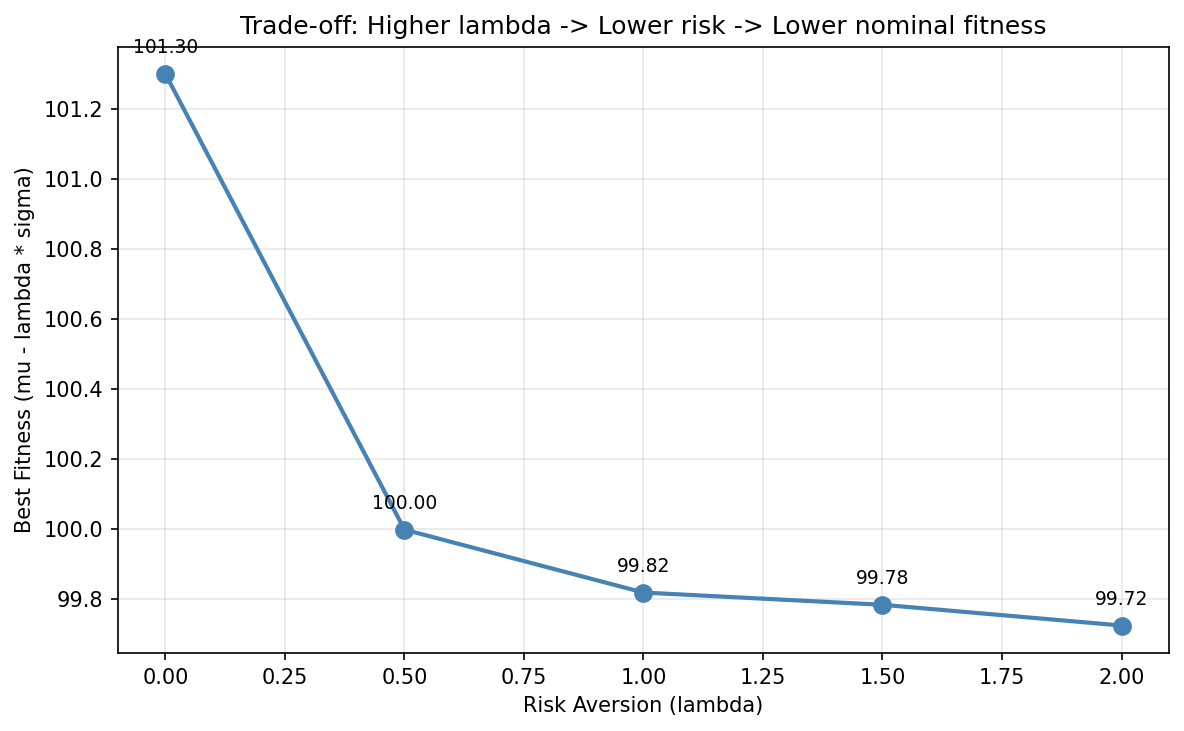
\includegraphics[width=0.72\textwidth]{figures/lambda_vs_stability.png}
\caption{不同风险系数 $\lambda$ 下的最优适应度——$\lambda=0$ 时越过理论上限 100}
\label{fig:lambda}
\end{figure}

稳定性评分的物理上限是 100。当以纯均值 $\mu(x)$ 为目标
（即第~\ref{sec:risk}~节风险敏感公式取 $\lambda=0$）寻优时，
PSO 报告的最优适应度达到 \textbf{101.30}（图~\ref{fig:lambda}）。
由于此时适应度即为 $\mu(x)$，$101.30$ 表明代理输出了 $\mu(x)>100$
的、无物理意义的预测值。这是典型的代理模型过度外推（Extrapolation）：
优化器将粒子推至训练数据稀疏的区域，代理在该区域产生明显的过度外推。

\subsection{异常二：不同优化器给出几乎相同的解}

改用遗传算法（GA）、差分进化（DE）、模拟退火（SA）在同一代理上寻优。
通常机制不同的优化器在复杂景观中应得到不同的局部解。
但实测（第~\ref{sec:converge}~节表~\ref{tab:ci_comparison}）显示，
PSO、GA、DE 的最优适应度集中在 $100.14$--$100.29$ 的极窄区间，
\textbf{极差仅 0.15}，即更换优化算法几乎不改变结果。

\subsection{异常三：不同赛道场景给出高度相似的解}

进一步定义四组差异较大的赛道工况（Monza 极速、Monaco 高下压、均衡、湿地），
赋予差异显著的多目标权重，分别寻优。
结果（第~\ref{sec:converge}~节表~\ref{tab:scenario_opt}）显示：
\textbf{各场景的翼角均收敛到约 $20^\circ$、阻力均收敛到下界 18 N}，
场景差异几乎只体现在被硬约束固定的速度与 DRS 上，
不同场景的最优解高度趋同。

\begin{figure}[H]
\centering
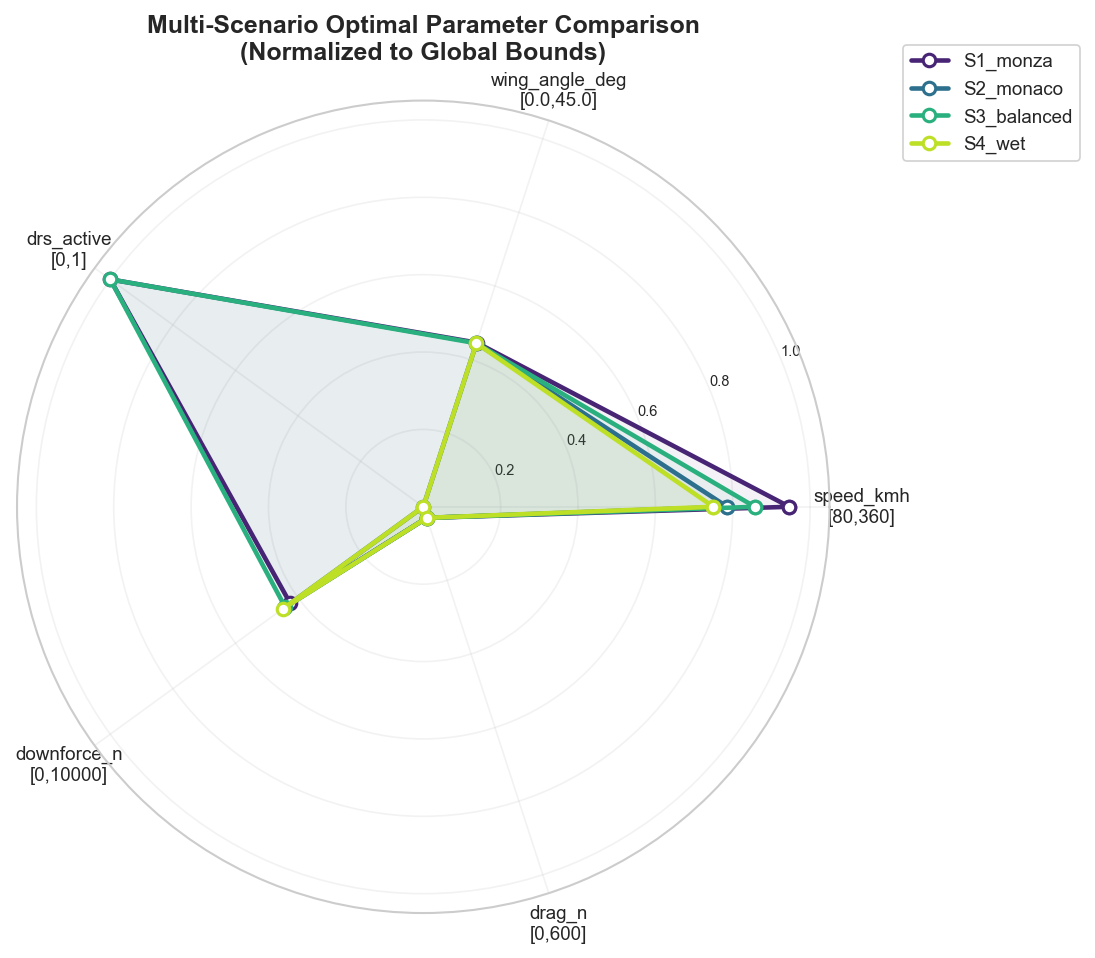
\includegraphics[width=0.72\textwidth]{figures/07_scenario_radar.png}
\caption{不同场景下最优解的参数分布}
\label{fig:radar}
\end{figure}

\subsection{小结：准确性与可信性的差异}

上述三项异常无法由"代理预测精度不足"解释——代理的预测精度很高
（第~\ref{sec:surrogate}~节）。由此提出后续研究的核心问题：

\begin{chapterquestion}
在代理模型预测精度很高的前提下，优化结果为何仍出现越过物理上限、
且对优化算法与赛道场景均不敏感的异常？
\end{chapterquestion}

回答该问题，需将研究目标从"预测是否准确"转向"预测是否可信"。
第~\ref{sec:uncertainty}~节引入用于度量可信度的预测不确定性 $\sigma(x)$。
